% This is samplepaper.tex, a sample chapter demonstrating the
% LLNCS macro package for Springer Computer Science proceedings;
% Version 2.20 of 2017/10/04
%
\documentclass[runningheads]{llncs}
%
\usepackage{graphicx}
\usepackage{amsmath}
\usepackage{amsfonts}
\usepackage{float}
% Used for displaying a sample figure. If possible, figure files should
% be included in EPS format.
%
% If you use the hyperref package, please uncomment the following line
% to display URLs in blue roman font according to Springer's eBook style:
% \renewcommand\UrlFont{\color{blue}\rmfamily}

\begin{document}
%
\title{Dual watermarking scheme for handwritten document image integrity, tamper detection and copyright protection}
%
%\titlerunning{Abbreviated paper title}
% If the paper title is too long for the running head, you can set
% an abbreviated paper title here
%
\author{Ernesto Avila-Domenech\inst{1}\orcidID{0000-0002-4797-289X} \and
Alberto Taboada-Crispi\inst{2}\orcidID{0000-0002-7797-1441} \and
Anier Soria-Lorente\inst{1}\orcidID{0000-0003-3488-3094}}
%
\authorrunning{E. Avila-Domenech et al.}
% First names are abbreviated in the running head.
% If there are more than two authors, 'et al.' is used.
%
\institute{Universidad de Granma, Carretera Central v{\'i}a Holgu{\'i}n Km $\frac{1}{2}$, Granma, Cuba \email{\{eadomenech, asorial1983\}@gmail.com}\\ \and
Universidad Central de Las Villas, Villa Clara, Cuba\\
\email{\{abc,lncs\}@uni-heidelberg.de}}
%
\maketitle              % typeset the header of the contribution
%
\begin{abstract}
For the integrity, tamper detection and copyright protection of handwritten document images, a dual watermarking algorithm that connects the robust watermarking algorithm based on Neural Network with a fragile watermarking algorithm based on SHA-256 hash function is presented. Hence, the robust watermarking algorithm is used to guarantee stability and robustness by modifying frequency coefficients in Krawtchouk moments. Thus, this study proposes a fragile watermarking algorithm, which can perceive in time when the protected image is tampered. Experimental results show that the proposed algorithm can be used for copyright protection and tampering detection of this images.

\keywords{First keyword  \and Second keyword \and Another keyword.}
\end{abstract}
%
%
%
\section{Introduction}
The explosive growth of digital multimedia techniques, together with the rapid development of digital network communication has created a pressing demand for techniques that can be used for copy protection, copyright protection and content authentication. Owing to the need of copyright protection and authentication validation, Digital Rights Management (DRM) is gaining importance. DRM refers to a range of access control technologies used to limit or restrict usage of digital content. Digital watermarking is useful in DRM systems as it can hide information within the digital content like images, audio and video.

Watermarking technique is effectively applied to content authentication, integrity protection, and image copyright. In accordance with the desired robustness of the embedded watermark, digital watermarking techniques are divided into robust watermarking and fragile watermarking. The first ones is designed to detect slight changes to the watermarked image with high probability and the second ones is typically used for copyright protection, thus it is designed to resist attacks that attempt to remove or destroy the watermark without significantly degrading the visual quality of the watermarked image.

When users want to protect the copyright and at the same time detect illegal tampering, the single watermarking algorithm cannot meet the needs of users. Therefore, the double watermarking algorithm is developed, as it can effectively combine the advantages and functions of the two watermarks \cite{wang2017dual}.

Numerous double watermarking algorithms have been proposed. In \cite{mohanty1999dual} is presented a dual watermarking technique which attempts to establish the owner’s right to the image and detect the intentional and unintentional tampering of the image. However, this early research is simply a combination of visible and invisible watermarking algorithms. In \cite{wang2017dual} is presents a dual watermarking algorithm that connects the robust watermarking algorithm based on singular value decomposition (SVD) with a fragile watermarking algorithm based on compressive sensing (CS). In \cite{singh2018hybrid} use cryptography and QR Code in combined approach of LSB and DCT Digital image watermarking technique, it combines the LSB and DCT approach because LSB contain spatial domain property and DCT contain frequency domain property.

In \cite{liu2018blind} presents a blind dual watermarking mechanism for digital color images. The first watermark is embedded by using the discrete wavelet transform (DWT) in YCbCr color space, and it can be extracted blindly without access to the host image. However, fragile watermarking is based on an improved least significant bits (LSB) replacement approach in RGB components for image authentication. In \cite{singh2019robust} presents lifting wavelet transform (LWT) and discrete cosine transform (DCT) based robust watermarking approach for tele-health applications. They are based on LWT requires less memory, reduced aliasing effects and distortion, fast and it is a good choice for low computational complexity than conventional DWT.

In \cite{gul2019novel} host image is divided into $32\times 32$ non-overlapped blocks, each $32\times 32$ block is then divided into four $16\times 16$ nonoverlapped sub-blocks. The entire hash value of the first three sub-blocks is generated as a watermark using SHA-256 hash function. The generated 256-bit binary watermark is embedded into the least significant bits (LSBs) of the fourth sub-block and watermarked image is obtained.

Deep learning is a new area of machine learning which has gained popularity in recent past. Deep learning refers to the architectures which contain multiple hidden layers (deep networks) to learn different features with multiple levels of abstraction. Deep learning algorithms seek to exploit the unknown structure in the input distribution in order to discover good representations, often at multiple levels, with higher level learned features defined in terms of lower level features. \cite{wani2019advances}

Different from previous works \cite{avila2018watermarking}, an effective algorithm that effectively utilizes spatial context to classify the $8\times 8$ blocks according to the optimal marking parameters is proposed in this paper. For capturing spatial information of $8\times 8$ blocks, a neural network was used in our technique, which has been proven to be effective in classification tasks.

The rest of the paper is organised as follow; Section 2 describes the proposed method including fragil watermarking and robust watermarking. Experimental results are given in Section 3 and Section 4 concludes the paper.

\section{Proposed method}
As we know, hash function, such as MD5 or SHA-256, can be utilized to authenticate the data integrity. If the hash value of original message is exactly equal to the re-calculated hash value of the received message, the received data can be regarded as integrated, otherwise as false.

\subsection{Robust watermarking}
The robust watermarking method proposed is similar to the one proposed in \cite{avila2018watermarking}. The difference consists in using a neural network topology known as multilayer perceptron (MLP) to classify the $8\times 8$ blocks according to the optimal marking parameters. A MLP is a feed-forward net with one or more layers of nodes between the input and output nodes. These in-between layers are called hidden layers.

Training is equivalent to finding proper weights for all the connections such that a desired output is generated for a corresponding input. Using MLP in the context of a classifier requires all output nodes to be set to 0 except for the node that is marked to correspond to the class the input is from. That desired output is 1. 

The most important step in solving any real-world problem is to get the data. Kaggle provides a huge number of competitions on different data science problems \cite{Subramanian2018}.

For that, a new dataset of $8\times 8$ color images of 70000 fashion products from 10 categories, with 7, 000 images per category was create. The training set has 60000 images and the test set has 10000 images. The dataset was obtained by dividing into $8\times 8$ blocks each of the images corresponding to the DIBCO 2017 dataset and calculating the coef and delta values so that the balance between PSNR and BER represented as $FO$ were the highest possible values for each of the blocks.
\begin{equation}
FO = (PSNR/160 + \alpha + \beta)/3,
\label{FA}
\end{equation}
where $PSNR$ is the logarithmic value of ratio between signal and noise, $ \alpha $ is the success in extracting the watermark from the watermarked image without noise and $ \beta $ is the success in extracting the watermark from the watermarked image after applying a JPEG compression with QF= 25{\%}.

The network was trained using GPU NVIDIA GTX 780ti for a week. 

In this process we use an open-source machine learning library for Python PyTorch \cite{paszke2017pytorch}. PyTorch extensively uses Python concepts, such as classes, structures, and conditional loops, allowing us to build Deep Learning algorithms in a pure object-oriented fashion. Most of the other popular frameworks bring their own programming style, sometimes making it complex to write new algorithms and it does not support intuitive debugging. What makes PyTorch increasingly popular is its ease of use and simplicity \cite{Subramanian2018}.

Once the model is trained, the following steps are taken to complete the insertion process:
\begin{enumerate}
	\item The binary watermark image (QR code) is scrambled using Arnold transform \cite{Arnol'd:1987366}.
	\item The cover image is transformed from RGB to YCbCr color space, and the Y component, corresponding to the luminance information, is divided into small image blocks of $8\times 8$ pixels.
	\item The Krawtchouk moments \cite{Yap2003} of selected blocks are determined.
	\item Each selected block is classified by the model previously trained in one of the defined classes.
	\item Watermark bit is embedded in the selected block moments using Dither modulation \cite{chen2001quantization}. Both the coefficient and the delta value are obtained according to the class that has been classified each block. Watermarked blocks can be obtained. 
	\item Transform the YCbCr to RGB color space to obtain RGB watermarked image.
\end{enumerate}

For watermark extraction:
\begin{enumerate}
	\item The watermarked image is transformed from the RGB to the YCbCr color space and the Y component is divided into $8\times 8$ pixels blocks.
	\item The Krawtchouk moments of selected blocks are determined.
	\item Each selected block is classified by the model previously trained in one of the defined classes. According to the class, the coefficient and delta to be used in the extraction are determined.
	\item Scrambled watermark bits are obtained with the selected blocks moments using Dither modulations.
	\item Finally, QR code watermark is constructed with the scrambled bits using Arnold transform.
\end{enumerate}

\subsection{Fragile watermarking}
For the embedding process, the image is divided into $32\times 32$ non-overlapped blocks. The complete block is pariado making use of a given key. The entire hash value of the block pariado is generated as a watermark using MD5 hash function. The generated MD5 binary watermark is embedded into the least significant bits (LSBs) of the pixels pariados and watermarked image is obtained.

The detection of a fragile watermark is the inverse process of watermark generation, which is used to detect whether the watermarked image has been tampered and what the precise position of the tampered parts is. For this, the watermarked image is divided into $32\times 32$ non-overlapped blocks. The complete block is pariado making use of a given key. The entire hash value of the block pariado is calculate and ...

\section{Experiments and Results}
The watermarking algorithm is evaluated through imperceptibility, tamper detection and robustness, and the following experiments are introduced.
 

\subsection{Imperceptibility}
The imperceptibility of the watermark was evaluated using several databases. We calculated the larger peak signal to noise ratio (PSNR) which compares the similarity between the original image $ I $ and the watermarked image $ I_w $. A PSNR indicates that the watermarked image more closely resembles the original image meaning that the watermark is more imperceptible.

\subsection{Tamper detection}
Tamper area detection capability is evaluated, by modifying the contents of images, adding objects or deleting objects.

\begin{figure}[h]
	\begin{center}
		\begin{tabular}{|c|c|c|c|}\hline
			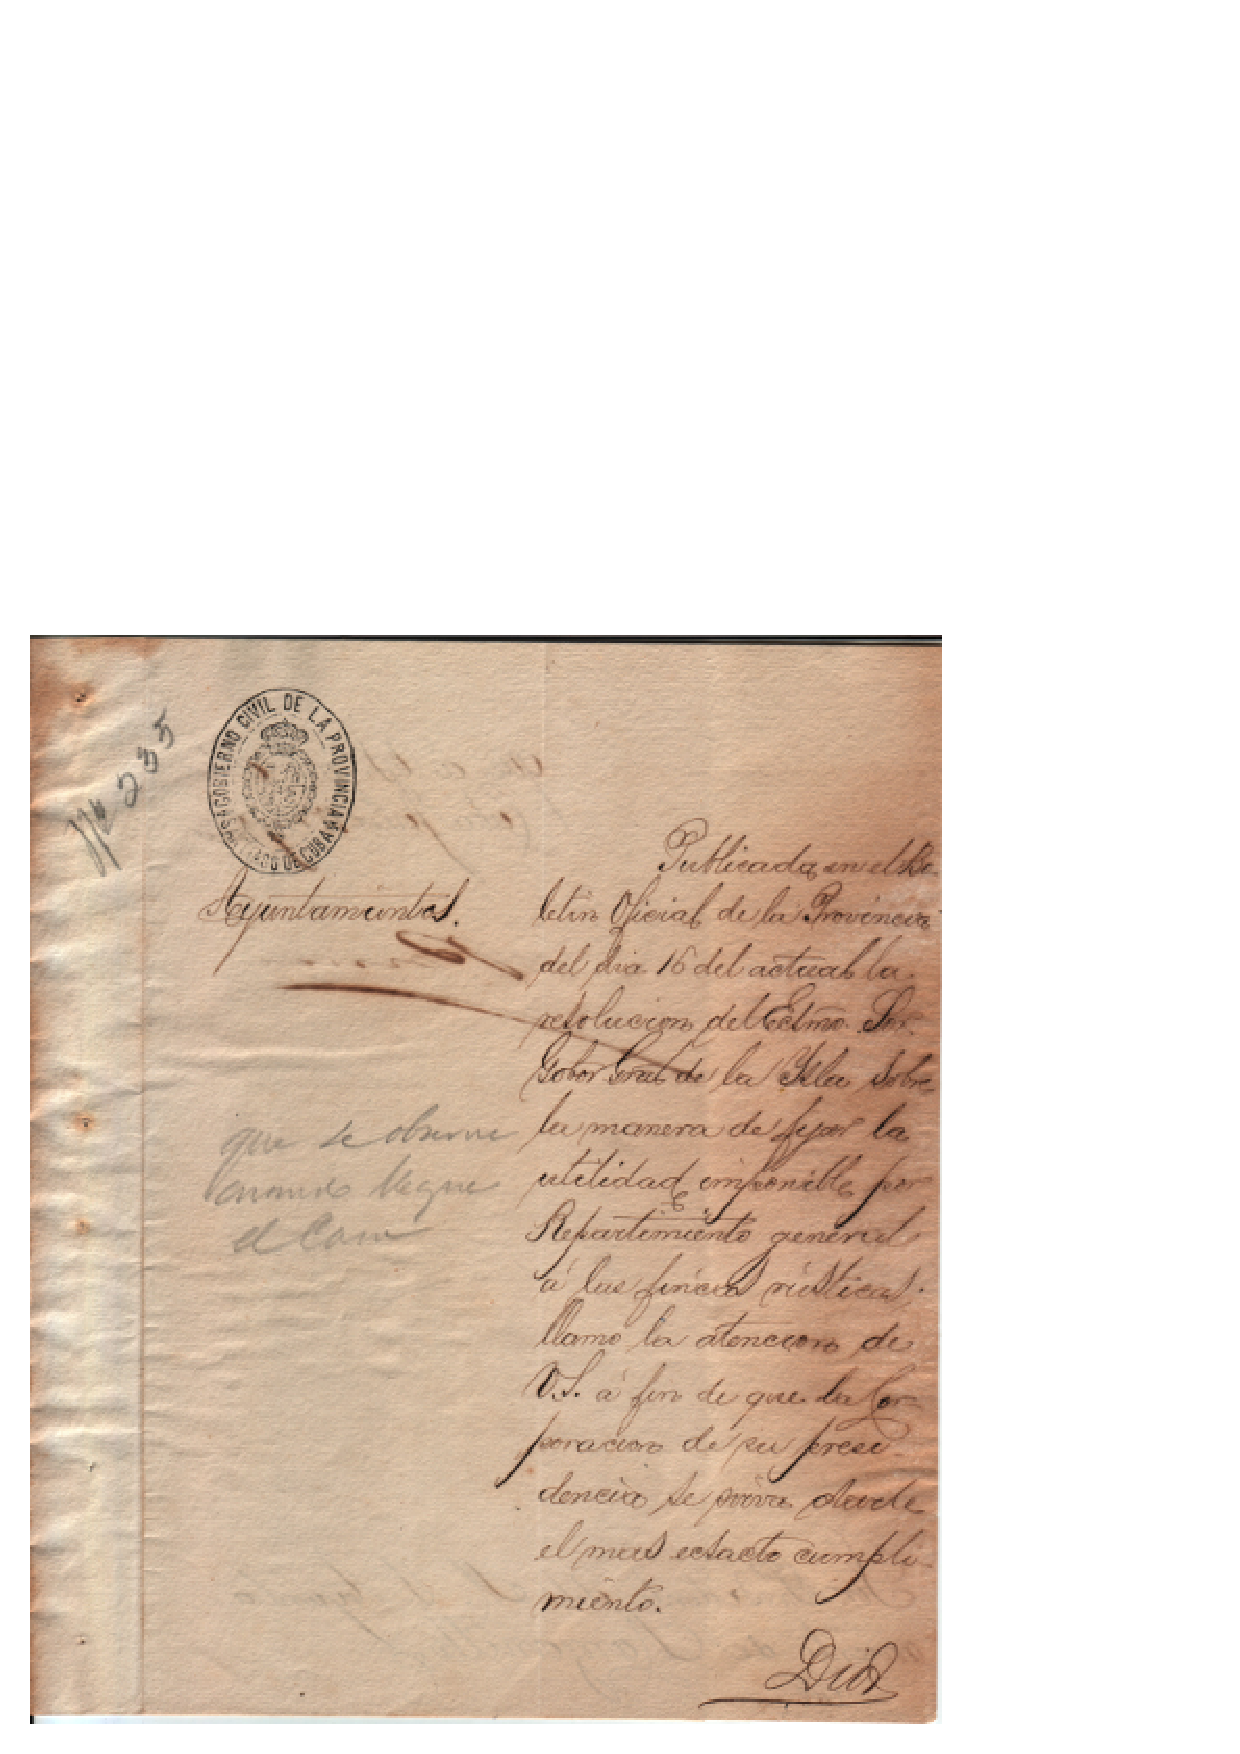
\includegraphics[width=0.25\textwidth]{1.jpg}
			&\includegraphics[width=0.25\textwidth]{watermarked_image.png}
			&\includegraphics[width=0.25\textwidth]{watermarked_image_with_noise.png}
			&\includegraphics[width=0.25\textwidth]{tampered_image.png}\\\hline
		\end{tabular}
	\end{center}
	\caption{Original image, watermarked image (PSNR 62.06), watermarked modified image and tamper area detection.}
	\label{img_of_AHM}
\end{figure}

\subsection{Robustness}
The bit error rate (BER) is defined as ratio between number of incorrectly decoded bits and total number of bits.

\begin{table}
\caption{Table captions should be placed above the
tables.}\label{tab1}
\begin{tabular}{|l|l|l|}
\hline
Heading level &  Example & Font size and style\\
\hline
Title (centered) &  {\Large\bfseries Lecture Notes} & 14 point, bold\\
1st-level heading &  {\large\bfseries 1 Introduction} & 12 point, bold\\
2nd-level heading & {\bfseries 2.1 Printing Area} & 10 point, bold\\
3rd-level heading & {\bfseries Run-in Heading in Bold.} Text follows & 10 point, bold\\
4th-level heading & {\itshape Lowest Level Heading.} Text follows & 10 point, italic\\
\hline
\end{tabular}
\end{table}


\noindent Displayed equations are centered and set on a separate
line.
\begin{equation}
x + y = z
\end{equation}
Please try to avoid rasterized images for line-art diagrams and
schemas. Whenever possible, use vector graphics instead (see
Fig.~\ref{fig1}).

\begin{figure}
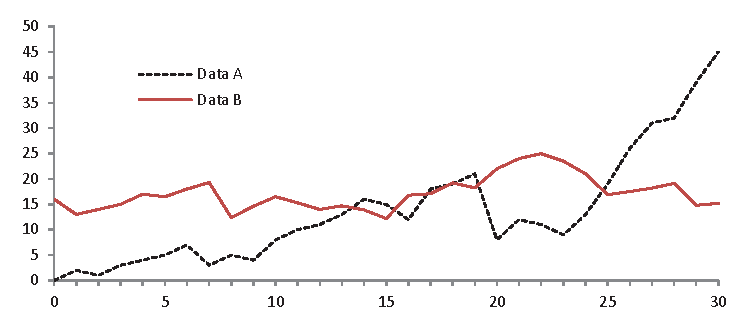
\includegraphics[width=\textwidth]{fig1.eps}
\caption{A figure caption is always placed below the illustration.
Please note that short captions are centered, while long ones are
justified by the macro package automatically.} \label{fig1}
\end{figure}

\begin{theorem}
This is a sample theorem. The run-in heading is set in bold, while
the following text appears in italics. Definitions, lemmas,
propositions, and corollaries are styled the same way.
\end{theorem}
%
% the environments 'definition', 'lemma', 'proposition', 'corollary',
% 'remark', and 'example' are defined in the LLNCS documentclass as well.
%
\begin{proof}
Proofs, examples, and remarks have the initial word in italics,
while the following text appears in normal font.
\end{proof}
\section{Conclusions}
In this paper, a digital watermarking technique based on Krawtchouk moments was implemented, and it was optimized by a genetic algorithm for manuscript document images. The results show a BER less than $0.005 \%$, so the extracted QR codes were decoded in $100\%$ of the $60$ analyzed images. In addition, the values of PSNR in all cases exceeded $44dB$. Thus, there is no visual difference between the original and watermarked images.

\section{Acknowledgment}
The National Biotechnology Center is thanked, especially the researcher Yunior Cesar Fonseca Reyna belonging to the Department of Structure Macromolecules for his help in the training of the algorithm.
%
% ---- Bibliography ----
%
% BibTeX users should specify bibliography style 'splncs04'.
% References will then be sorted and formatted in the correct style.
%
\bibliographystyle{splncs04}
\bibliography{mybibliography}
%
\end{document}
